\documentclass[10pt]{article}

\usepackage[a4paper,margin=22mm]{geometry}
\usepackage{amsmath,amssymb}
\usepackage{booktabs}
\usepackage{graphicx}
\usepackage{tabularx}
\usepackage{array}
\usepackage{enumitem}
\usepackage{xcolor}
\usepackage{microtype}
\usepackage[hidelinks]{hyperref}
\usepackage[font=small,labelfont=bf]{caption}

\graphicspath{{figs/}}
\setlength{\parindent}{0pt}
\setlength{\parskip}{4pt}
\setlist{nosep,leftmargin=*}
\setlength{\tabcolsep}{4pt}
\newcolumntype{Y}{>{\raggedright\arraybackslash}X}
\newcolumntype{Z}{>{\centering\arraybackslash}X}
\newcolumntype{P}[1]{>{\centering\arraybackslash}p{#1}}

\title{CIFAR-100 Image Classification with a Designed Convolutional Network}
\author{}
\date{}

\begin{document}
\maketitle

\begin{abstract}
This course-work report presents Part A of a two-part deep-learning project. It studies a complete CIFAR-100 image-classification pipeline, from a deliberately simple convolutional baseline to a custom wide residual network. The accuracy is improved step by step by stabilizing optimization, adding normalization and a warmup--cosine schedule, redesigning the spatial hierarchy, increasing capacity, and training with appropriate augmentation. The main conclusion is that augmentation is budget-dependent and that width plus residual depth is more reliable than depth alone. After retraining on all 50,000 training images, the best result is 77.87\% top-1 accuracy from a three-model ensemble with horizontal-flip test-time augmentation.
\end{abstract}

\section*{Part A: PyTorch Image Classification}

\section{Introduction}

CIFAR-100 contains 60,000 colour images of size $32\times32$, distributed over 100 fine-grained classes and 20 superclasses \cite{krizhevsky}. The small spatial resolution makes the task a useful test of architectural choices: a network can easily memorize the training images while still lacking the capacity or inductive bias needed for good generalization. I therefore treated the work as a sequence of controlled comparisons rather than a search for one lucky configuration.

This course-work report first establishes a reference point with a four-layer $5\times5$ convolutional network. It then tests training stability and optimization choices, evaluates architectural changes including $3\times3$ stacks, spatial downsampling, width, depth, residual connections, depthwise-separable convolutions, and normalization, and finally retrains the selected configuration on the full training set. The result is interpreted through both aggregate accuracy and the structure of the remaining errors.

The controlled progression raises validation accuracy from 11.33\% for the short-budget SGD baseline to 74.13\% for the selected wide residual model at 60 epochs. After full-data retraining, the best three-model ensemble with horizontal-flip test-time augmentation reaches 77.87\% top-1 accuracy and 94.36\% top-5 accuracy.

\section{Environment and Training Protocol}

All models were implemented directly with PyTorch modules \cite{pytorch}. The experiments used Python 3.11.14, PyTorch 2.11.0 with CUDA 12.8, torchvision 0.26.0, and an NVIDIA RTX 4060 Laptop GPU with 8 GB memory. The controlled comparisons used float32 arithmetic. Automatic mixed precision (AMP) was measured separately as an engineering comparison and was not used to decide which model was better.

The CPU/GPU and AMP measurements are summarized in Table~\ref{tab:throughput}. The downsampled CNN reaches a $7.0\times$ GPU speed-up over the CPU. For the 20.7M-parameter final architecture, AMP reduces the step time from 164 ms to 87 ms, a $1.89\times$ speed-up, while peak allocated memory falls from 1,379 MB to 861 MB. These measurements explain why the longer experiments were feasible, but they do not change the accuracy comparisons.

\begin{table}[htbp]
\centering
\caption{Hardware and throughput measurements for a batch of 128.}
\label{tab:throughput}
\small
\begin{tabular}{@{}P{0.18\linewidth}P{0.20\linewidth}P{0.21\linewidth}P{0.18\linewidth}@{}}
\toprule
Device or mode & Model & Time per step (ms) & Images/s \\
\midrule
CPU, float32 & Downsampled & 185 & 691 \\
GPU, float32 & Downsampled & 27 & 4,838 \\
GPU, float32 & Final model & 164 & 780 \\
GPU, AMP & Final model & 87 & 1,471 \\
\bottomrule
\end{tabular}
\end{table}

The validation protocol used the same deterministic 45,000/5,000 train/validation split for every controlled experiment. Each reported multi-seed result averages seeds 0, 42, and 123; a single-seed screen is explicitly marked as such. The batch size was 128. The loss was cross-entropy. Unless stated otherwise, the optimizer was Adam \cite{adam} with learning rate $10^{-3}$ and a two-epoch linear warmup followed by cosine decay following the cosine-scheduling idea of \cite{sgdr}. The final retraining used all 50,000 training images and kept the 10,000-image test set untouched until training had finished. The complete settings are collected in Table~\ref{tab:settings}.

\begin{table}[htbp]
\centering
\caption{Common training settings.}
\label{tab:settings}
\small
\begin{tabular}{@{}P{0.18\linewidth}P{0.40\linewidth}P{0.30\linewidth}@{}}
\toprule
Setting & Controlled comparisons & Final retraining \\
\midrule
Data split & 45k train / 5k validation / 10k test & 50k train / 10k test \\
Batch size & 128 & 128 \\
Optimizer & Adam, $10^{-3}$ (SGD only for the reference) & Adam, $10^{-3}$ \\
Schedule & 2-epoch warmup + cosine decay & 2-epoch warmup + cosine decay \\
Epochs & 10, 20, or 60 & 60 \\
Augmentation & none or crop + horizontal flip & crop + horizontal flip \\
Seeds & 0, 42, 123 & 0, 42, 123 \\
\bottomrule
\end{tabular}
\end{table}

\section{Dataset and Preprocessing}

The input pipeline converts each image to a channel-first float tensor and normalizes it with the training-set statistics
\[
\mu=(0.5071,\ 0.4866,\ 0.4409),\qquad
\sigma=(0.2673,\ 0.2564,\ 0.2762).
\]
The validation and test transforms contain only tensor conversion and normalization. The augmented training transform adds a random crop to $32\times32$ with four-pixel padding and a random horizontal flip. No random transform is applied during evaluation. Figure~\ref{fig:data} shows denormalized training images with their labels; the grid was used to check channel order, image shape, and label alignment before training.

\begin{figure}[htbp]
\centering
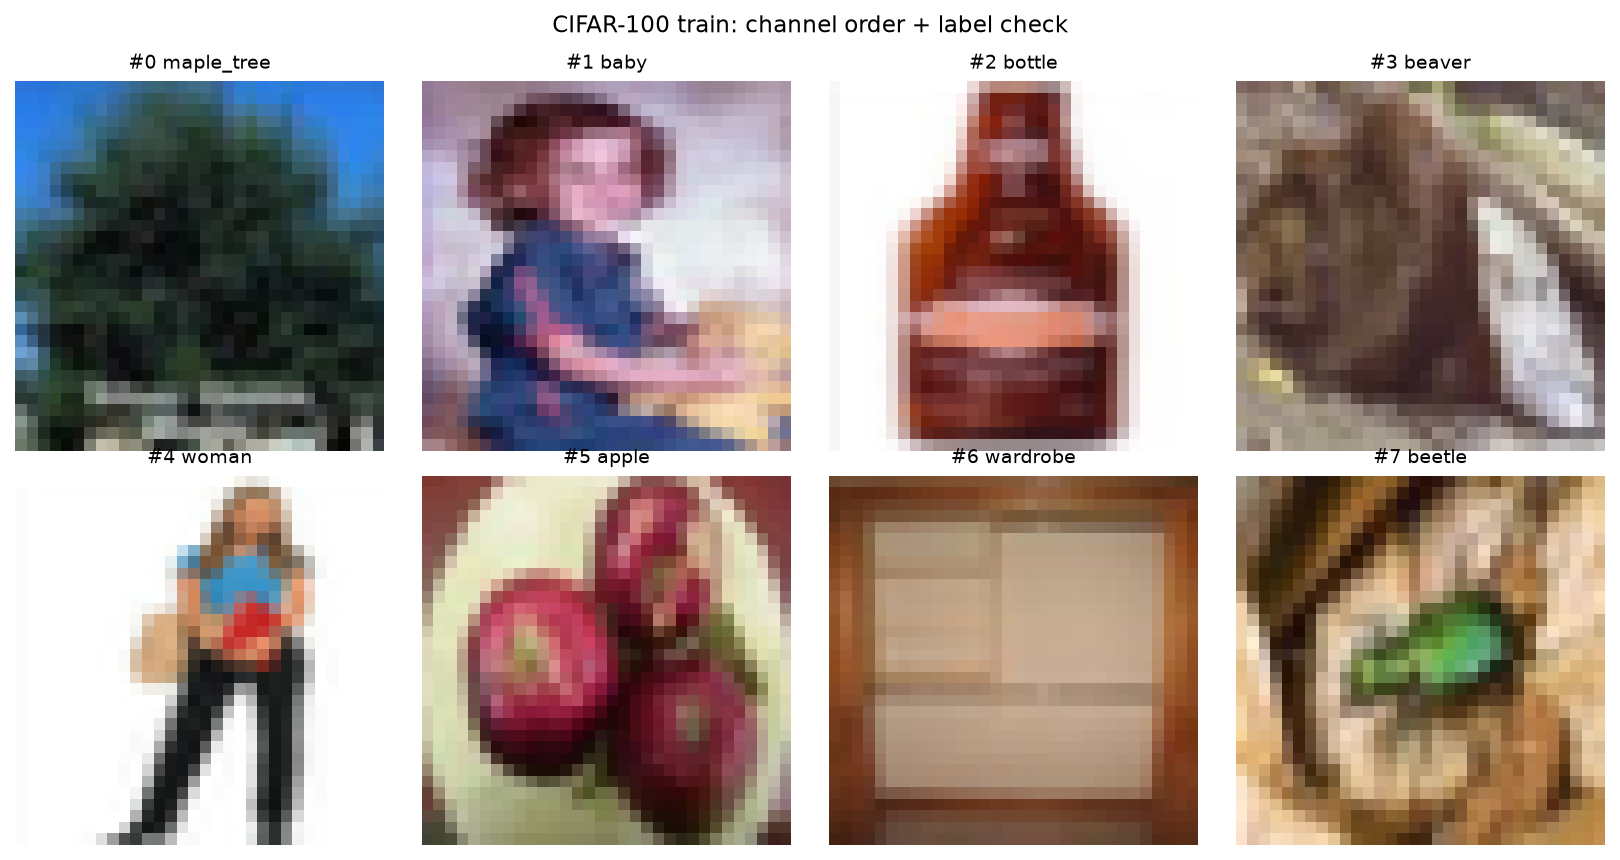
\includegraphics[width=0.96\linewidth]{data_samples.png}
\caption{Representative CIFAR-100 training images after reversing normalization for display. Each image is a $32\times32$ RGB tensor in channel-first form before plotting.}
\label{fig:data}
\end{figure}

\section{Baseline}

\subsection{Architecture}

The reference network keeps the spatial resolution at $32\times32$ through four convolutional layers:
\begin{equation}\label{eq:baseline}
\begin{aligned}
&\operatorname{Conv}(3,256,5)\rightarrow\operatorname{ReLU}\rightarrow
\operatorname{Conv}(256,256,5)\rightarrow\operatorname{ReLU}\\[-1pt]
&\qquad\rightarrow\operatorname{Conv}(256,256,5)\rightarrow\operatorname{ReLU}\rightarrow
\operatorname{Conv}(256,256,5)\rightarrow\operatorname{ReLU}\\[-1pt]
&\qquad\rightarrow\operatorname{GAP}\rightarrow\operatorname{Linear}(256,100).
\end{aligned}
\end{equation}
All convolutions use padding two. Equation~\ref{eq:baseline} has 4,961,124 trainable parameters. This is a useful reference because it is intentionally simple: it has no normalization, no downsampling, and no skip connections. The main architecture families are summarized in Table~\ref{tab:models}.

\begin{table}[htbp]
\centering
\caption{Architecture summary for the main model families.}
\label{tab:models}
\small
\begin{tabularx}{\linewidth}{@{}ZZZZZ@{}}
\toprule
Model & Stage widths & Strides & Main block & Parameters (M) \\
\midrule
Reference & $256,256,256,256$ & $1,1,1,1$ & four $5\times5$ convolutions & 4.96 \\
Downsampled & $64,128,256,256$ & $1,2,2,2$ & two $3\times3$ blocks/stage & 2.35 \\
Selected & $128,256,512,512$ & $1,2,2,2$ & two residual blocks/stage & 20.70 \\
\bottomrule
\end{tabularx}
\end{table}

\subsection{Ten-epoch result}

The baseline was trained for exactly 10 epochs with SGD and learning rate $10^{-2}$. The first row of Table~\ref{tab:short} is the reference. The remaining rows are a staged sequence in which the previous configuration is changed by one main factor at a time. Values are validation top-1 and top-5 accuracy in percent; the uncertainty is the standard deviation across three seeds.

\begin{table}[htbp]
\centering
\caption{Short-budget progression on the fixed 45k/5k validation split.}
\label{tab:short}
\small
\begin{tabular}{@{}P{0.46\linewidth}P{0.16\linewidth}P{0.16\linewidth}P{0.16\linewidth}@{}}
\toprule
Configuration & Augmentation & Top-1 (\%) & Top-5 (\%) \\
\midrule
Baseline + SGD & none & $11.33\pm0.30$ & $31.95\pm0.19$ \\
Baseline + Adam & none & $21.07\pm17.90$ & $42.11\pm27.15$ \\
Add BatchNorm & none & $47.17\pm0.25$ & $76.99\pm0.47$ \\
Add warmup + cosine decay & none & $54.09\pm0.11$ & $82.77\pm0.17$ \\
Add crop + flip & crop + flip & $49.93\pm0.18$ & $79.99\pm0.27$ \\
Replace $5\times5$ with stacked $3\times3$ & crop + flip & $54.25\pm0.43$ & $83.64\pm0.19$ \\
Downsampled $3\times3$ CNN & crop + flip & $61.00\pm0.68$ & $87.64\pm0.19$ \\
\bottomrule
\end{tabular}
\end{table}

The baseline curves in Figure~\ref{fig:baseline-curves} show that the ten-epoch model is still under-trained: the final training top-1 accuracy is only about 10\%. Replacing SGD with Adam improves the mean but produces a severe seed-dependent failure. One seed reaches only 0.76\% validation accuracy, while the other two reach 27.94\% and 34.52\%. BatchNorm removes this collapse and reduces the run-to-run spread from 17.90 percentage points to 0.25. The warmup--cosine schedule then gives the best short-budget result before architectural changes are introduced.

\begin{figure}[htbp]
\centering
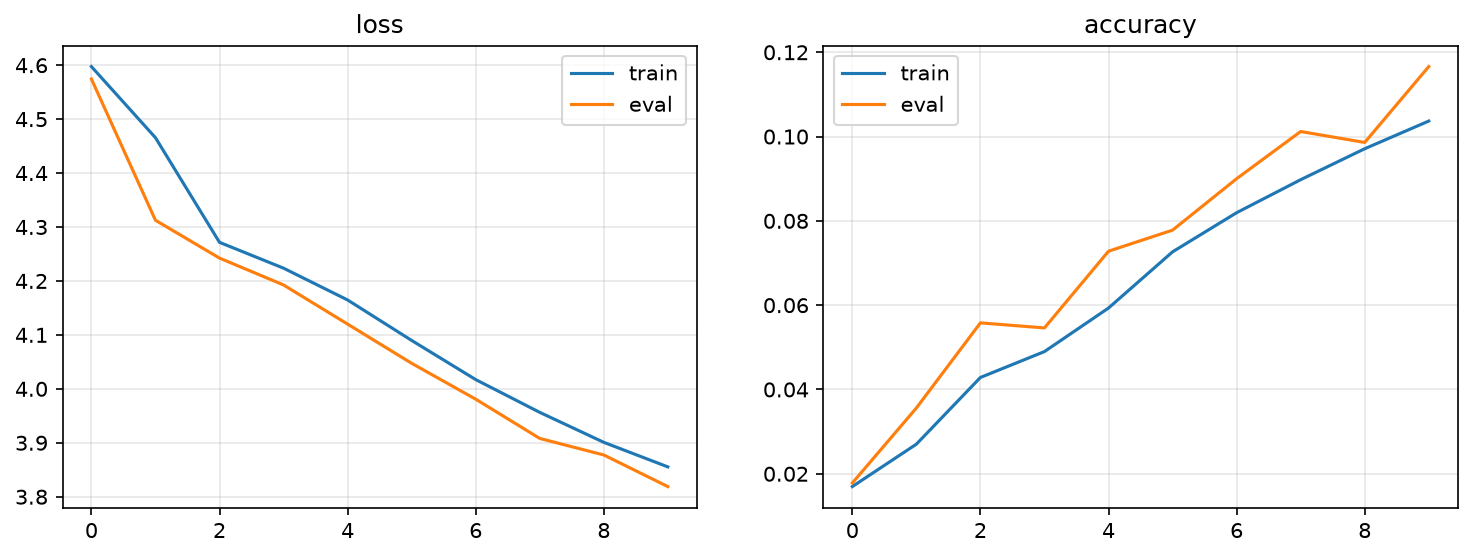
\includegraphics[width=0.96\linewidth]{baseline_curves.png}
\caption{Training and validation curves for one baseline seed over ten epochs. The slow but steady improvement confirms that the reference network is not yet fitting the training set.}
\label{fig:baseline-curves}
\end{figure}

\section{Experiments and Improvements}

\subsection{Experimental method}

The main comparisons use three distinct training budgets. The 10-epoch block establishes the reference and exposes optimization failures. The 20-epoch block screens architectural factors under a common augmented recipe. The 60-epoch block confirms promising factors and measures the effect of longer training. Keeping these budgets separate avoids attributing a gain from additional optimization steps to an architectural change.

For each comparison I recorded the motivation, changed one primary factor, measured validation accuracy, and retained both positive and negative results. This is particularly important for changes whose effect is smaller than the approximately one-percentage-point noise floor observed between repeated data-loader runs.

\subsection{Normalization, optimization, and spatial structure}

BatchNorm \cite{batchnorm} is the first major stability intervention. Without it, the combination of a high-dimensional input stem and Adam can produce an almost constant predictor for one random seed. With BatchNorm, the same seed reaches 47.04\% instead of 0.76\%. The warmup phase limits the initial update size, while cosine decay provides a smooth reduction of the learning rate after the network has entered a useful region.

The stacked $3\times3$ design has the same nominal receptive field as a $5\times5$ layer because two successive $3\times3$ kernels cover a $5\times5$ neighbourhood. It also introduces an additional nonlinearity and uses fewer weights for equal channel counts. The downsampled model goes further: it begins with 64 channels and uses stages with widths $(64,128,256,256)$ and strides $(1,2,2,2)$. Reducing spatial resolution makes later convolutions substantially cheaper and leaves capacity for more useful feature transformations. In the 10-epoch block, this model reaches 61.00\%, a gain of 6.91 points over the baseline.

\subsection{The role of augmentation and training duration}

Crop-and-flip augmentation is not uniformly beneficial at a short budget. At ten epochs it lowers the BatchNorm baseline from 54.09\% to 49.93\%. This is consistent with stronger regularization slowing memorization before the model has enough optimization time. The sign changes with a longer budget, as shown in Table~\ref{tab:aug-long}.

\begin{table}[htbp]
\centering
\caption{Effect of the same augmentation under a 60-epoch budget. All entries use three seeds and the 45k/5k validation split.}
\label{tab:aug-long}
\small
\begin{tabular}{@{}P{0.31\linewidth}P{0.21\linewidth}P{0.21\linewidth}P{0.15\linewidth}@{}}
\toprule
Architecture & No augmentation & Crop + flip & Difference \\
\midrule
Wide $\times2$ & $61.47\pm0.21$ & $72.48\pm0.33$ & $+11.01$ \\
Deep $\times2$ + residual & $58.13\pm0.05$ & $71.46\pm0.20$ & $+13.33$ \\
\bottomrule
\end{tabular}
\end{table}

The long-run curves show that the non-augmented wide models reach almost 100\% training accuracy early and then flatten or decline on validation data. Augmentation delays this memorization and continues to improve validation accuracy through the end of the 60-epoch schedule. Thus, the short-budget negative result does not contradict the long-budget positive result; the two measurements probe different stages of the optimization process.

\subsection{Architecture ablations}

The 20-epoch architecture screen is summarized in Table~\ref{tab:architecture-screen}. Every entry uses Adam, warmup--cosine decay, crop-and-flip augmentation, and batch size 128. The anchor is the downsampled CNN. Several changes are intentionally negative: depth alone, depthwise-separable convolution, and GroupNorm all reduce accuracy in this setting. Width is the strongest single variable, while depth becomes useful only after residual connections in the spirit of \cite{resnet} make the deeper optimization problem easier.

\begin{table}[htbp]
\centering
\caption{Architecture screen at 20 epochs. Single-seed screens are marked by $n=1$; the selected width and depth-plus-residual configurations were rechecked with three seeds.}
\label{tab:architecture-screen}
\small
\begin{tabular}{@{}P{0.60\linewidth}P{0.18\linewidth}P{0.12\linewidth}@{}}
\toprule
Change relative to the downsampled anchor & Validation top-1 (\%) & Seeds \\
\midrule
Downsampled anchor & 67.63 & $n=3$ \\
Residual connections only & 67.40 & $n=1$ \\
Width $\times2$ & $70.40\pm0.02$ & $n=3$ \\
Depth $\times2$ only & 64.52 & $n=1$ \\
Depth $\times2$ + residual connections & $69.15\pm0.50$ & $n=3$ \\
Remove the $4\times4$ stage & 63.12 & $n=1$ \\
Depthwise-separable convolutions & 54.58 & $n=1$ \\
Depthwise + compensating width & 65.00 & $n=1$ \\
GroupNorm instead of BatchNorm & 53.92 & $n=1$ \\
\bottomrule
\end{tabular}
\end{table}

The capacity comparison was then extended to 60 epochs. The final candidate combines width $\times2$, depth $\times2$, and residual connections. Its 20.7M parameters are spent on ordinary $3\times3$ convolutions rather than depthwise factorization. The resulting validation accuracy is 74.13\%, higher than either width-only or depth-only scaling, as summarized in Table~\ref{tab:long-architecture}. The first visualization below isolates the gain from each architectural factor and the change in the augmentation response.

\begin{table}[htbp]
\centering
\caption{Long-budget architecture comparisons at 60 epochs. All entries use crop-and-flip augmentation and three seeds.}
\label{tab:long-architecture}
\small
\begin{tabular}{@{}P{0.55\linewidth}P{0.18\linewidth}P{0.19\linewidth}@{}}
\toprule
Model & Parameters (M) & Validation top-1 (\%) \\
\midrule
Downsampled anchor & 2.35 & $69.40\pm0.31$ \\
Wide $\times2$ & 9.35 & $72.48\pm0.33$ \\
Deep $\times2$ + residual & 5.19 & $71.46\pm0.20$ \\
Deep $\times3$ + residual & 7.93 & $71.98\pm0.11$ \\
Deep $\times4$ + residual & 10.66 & $71.99\pm0.21$ \\
Wide $\times3$ & 21.00 & $73.40\pm0.41$ \\
Wide $\times2$ + deep $\times2$ + residual & 20.70 & $74.13\pm0.15$ \\
Wide $\times2$ + Cutout & 9.35 & $73.09\pm0.39$ \\
\bottomrule
\end{tabular}
\end{table}

Table~\ref{tab:long-architecture} shows the same pattern numerically: widening improves the score more consistently than adding residual depth, and the combined configuration gives the highest validation accuracy. Figure~\ref{fig:ablation} makes the incremental gains and their seed variability easier to compare.

\begin{figure}[htbp]
\centering
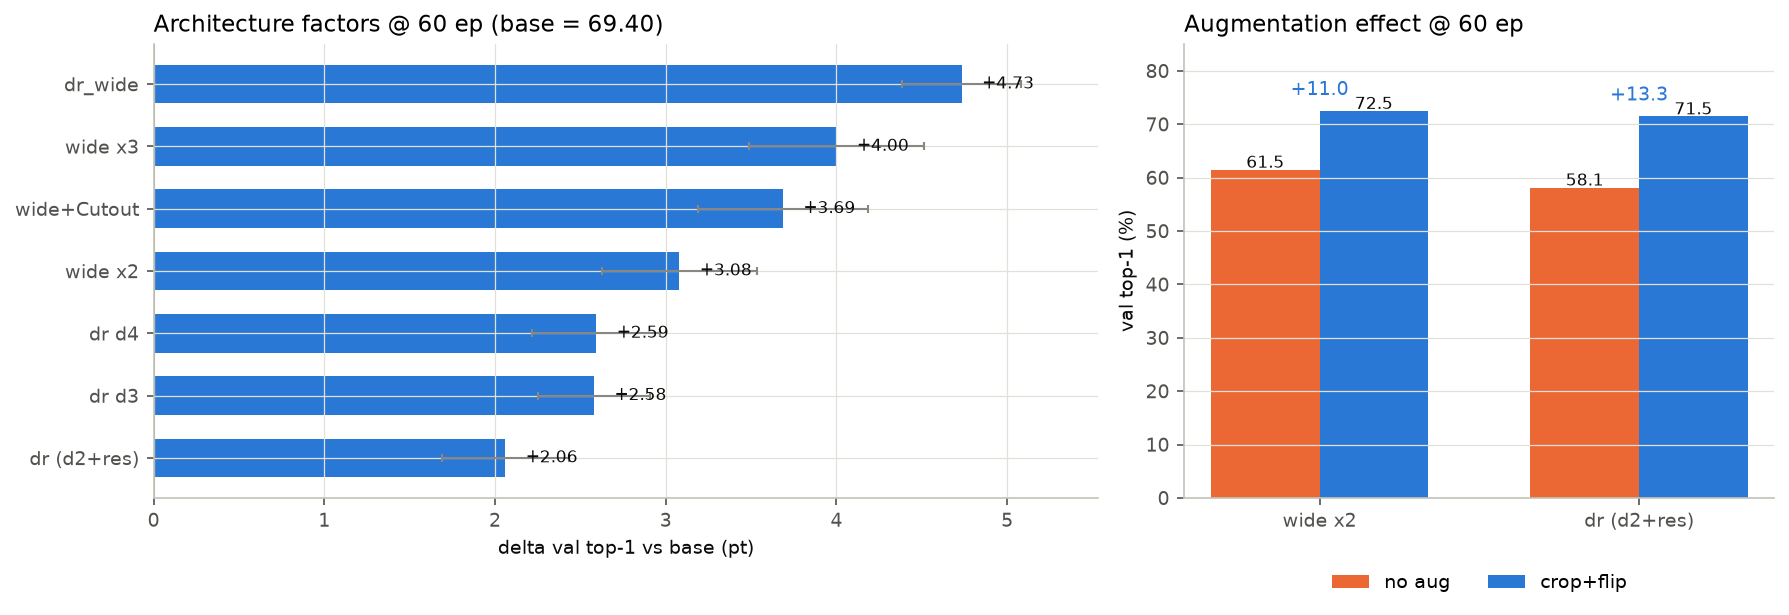
\includegraphics[width=0.99\linewidth]{ablation_60ep.png}
\caption{Validation gains at 60 epochs. The left panel compares architectural changes with the 2.35M-parameter anchor; the right panel isolates the augmentation effect for two architectures. Error bars show seed variability.}
\label{fig:ablation}
\end{figure}

The capacity plot in Figure~\ref{fig:capacity} complements Figure~\ref{fig:ablation}: width continues to improve the validation score over the tested range, whereas extra residual depth saturates after the third block per stage. This visual comparison is why the final model combines moderate depth with a wider channel schedule rather than using the deepest candidate.

\begin{figure}[htbp]
\centering
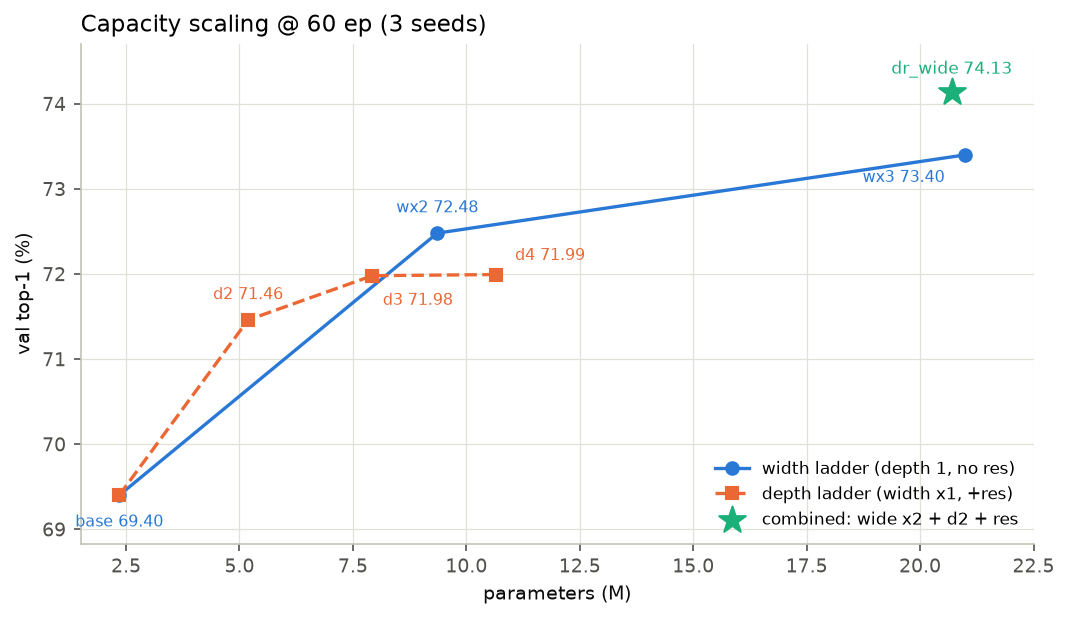
\includegraphics[width=0.86\linewidth]{capacity_scaling.png}
\caption{Width and depth capacity ladders at 60 epochs. Width keeps helping at the tested scales, whereas depth saturates after three residual blocks per stage. The star is the combined final candidate.}
\label{fig:capacity}
\end{figure}

\subsection{Selected model and training curve}

The selected architecture has four stages with widths $(128,256,512,512)$ and strides $(1,2,2,2)$. Each stage contains two residual blocks, and each block contains two $3\times3$ convolutions with BatchNorm and ReLU. A $1\times1$ projection is used in a shortcut whenever the spatial size or channel count changes. Global average pooling and a 100-way linear classifier produce the logits. This design has 20,702,308 trainable parameters.

Figure~\ref{fig:final-curves} displays one 60-epoch validation run. The raw validation accuracy rises from 22.76\% to 74.20\%, while the EMA curve provides a smoother mid-training estimate. The raw and EMA curves converge near the end of cosine decay, so the final comparison uses the raw model weights.

\begin{figure}[htbp]
\centering
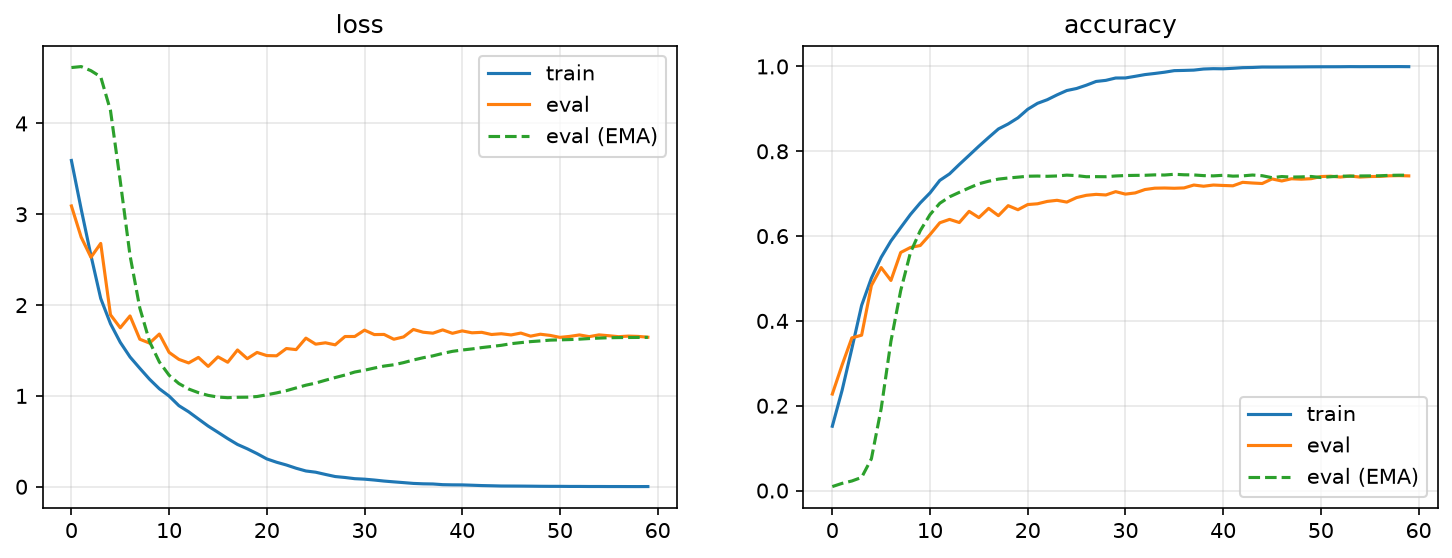
\includegraphics[width=0.96\linewidth]{final_val_curves.png}
\caption{Training and validation curves for one seed of the selected model on the 45k/5k protocol. The dashed curve is an exponential moving average used for monitoring.}
\label{fig:final-curves}
\end{figure}

\section{Final Model and Error Analysis}

After model selection on the validation protocol, the selected architecture was retrained for 60 epochs on all 50,000 training images for seeds 0, 42, and 123. The test set was evaluated after training. Test-time augmentation (TTA) averages the predictions for the original image and its horizontal flip. The three-seed ensemble averages class probabilities before taking the prediction. The resulting test metrics are listed in Table~\ref{tab:final-test}.

\begin{table}[htbp]
\centering
\caption{Final test-set results after full-data retraining.}
\label{tab:final-test}
\small
\begin{tabular}{@{}P{0.50\linewidth}P{0.19\linewidth}P{0.19\linewidth}@{}}
\toprule
Evaluation & Top-1 (\%) & Top-5 (\%) \\
\midrule
Single model, mean $\pm$ std & $75.01\pm0.32$ & $93.24\pm0.03$ \\
Single model + TTA, mean $\pm$ std & $75.69\pm0.33$ & $93.48\pm0.13$ \\
Three-model ensemble & 77.57 & 94.12 \\
Three-model ensemble + TTA & \textbf{77.87} & \textbf{94.36} \\
\bottomrule
\end{tabular}
\end{table}

The single-model result is already 0.88 points above the 45k/5k validation estimate, while probability averaging contributes a further 2.56 points over the single-model mean. TTA adds 0.30 points to the ensemble top-1 score. All four evaluation modes are reported because they measure different deployment choices.

\subsection{Superclass-level confusion}

For interpretable error analysis, I aggregated the 100 fine classes into the 20 CIFAR-100 superclasses using the dataset metadata. The confusion matrix in Figure~\ref{fig:confusion} is computed from the three-model ensemble without TTA, whose top-1 accuracy is 77.57\%. It contains 2,243 errors, of which 812 (36.2\%) remain inside the correct superclass. Among wrong predictions, a uniform classifier would place only about $4/99\approx4\%$ in the correct superclass, so the errors are strongly concentrated among semantically related categories.

The most frequent confusions include boy $\rightarrow$ man (18), oak tree $\rightarrow$ maple tree (16), girl $\rightarrow$ woman (16), otter $\rightarrow$ seal (13), and maple tree $\rightarrow$ oak tree (13). The diagonal structure at the superclass level indicates that the model has learned useful coarse semantics even when fine-grained visual distinctions remain difficult.

\begin{figure}[htbp]
\centering
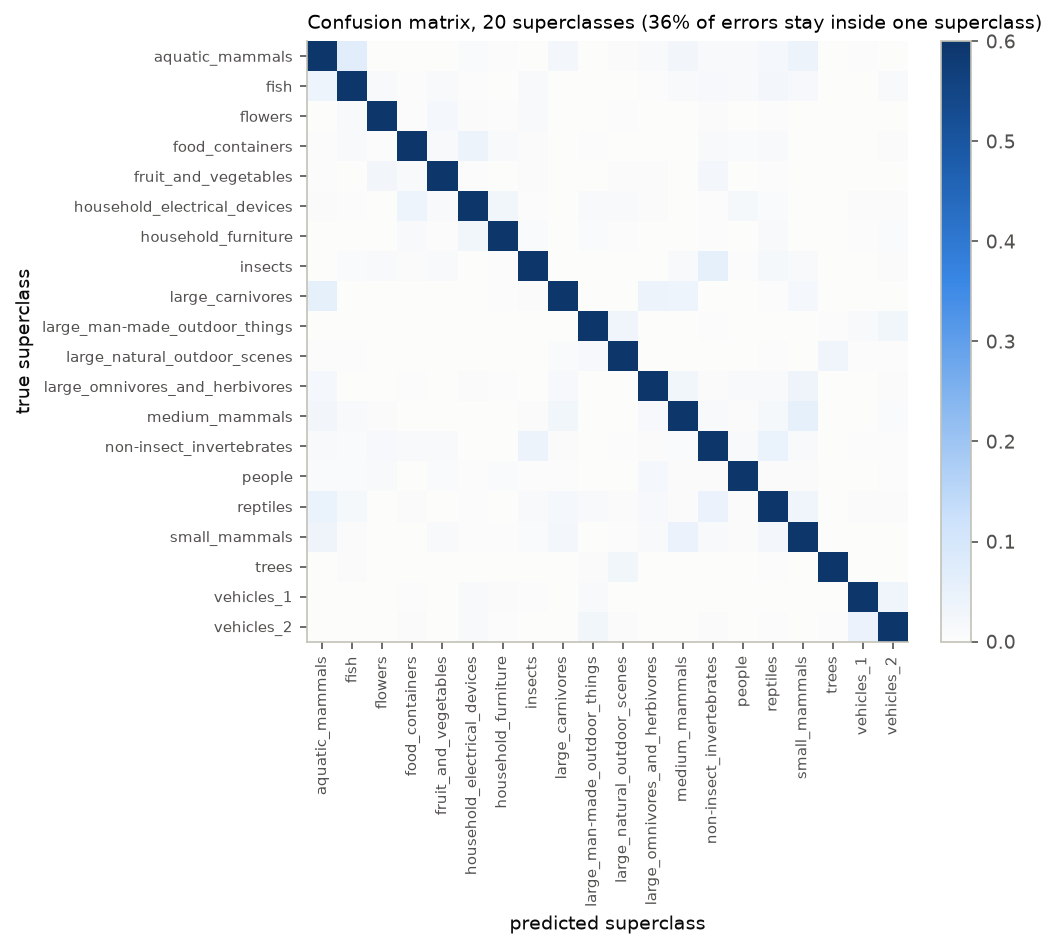
\includegraphics[width=0.82\linewidth]{confusion_coarse.png}
\caption{Row-normalized confusion matrix aggregated over the 20 superclasses. The diagonal is strong, while the remaining mass is concentrated in semantically close groups.}
\label{fig:confusion}
\end{figure}

\subsection{Per-class accuracy and representative errors}

Figure~\ref{fig:per-class} sorts the 100 fine classes by accuracy. The weakest classes are boy (48\%), girl (53\%), otter (54\%), bowl (57\%), and seal/possum (59\%). The strongest classes are tractor (97\%), motorcycle (96\%), and plain, wardrobe, and orange (94\%). The gap is consistent with the confusion matrix: object categories with distinctive shapes are easier than small, low-resolution classes that share colour and texture with nearby categories.

\begin{figure}[htbp]
\centering
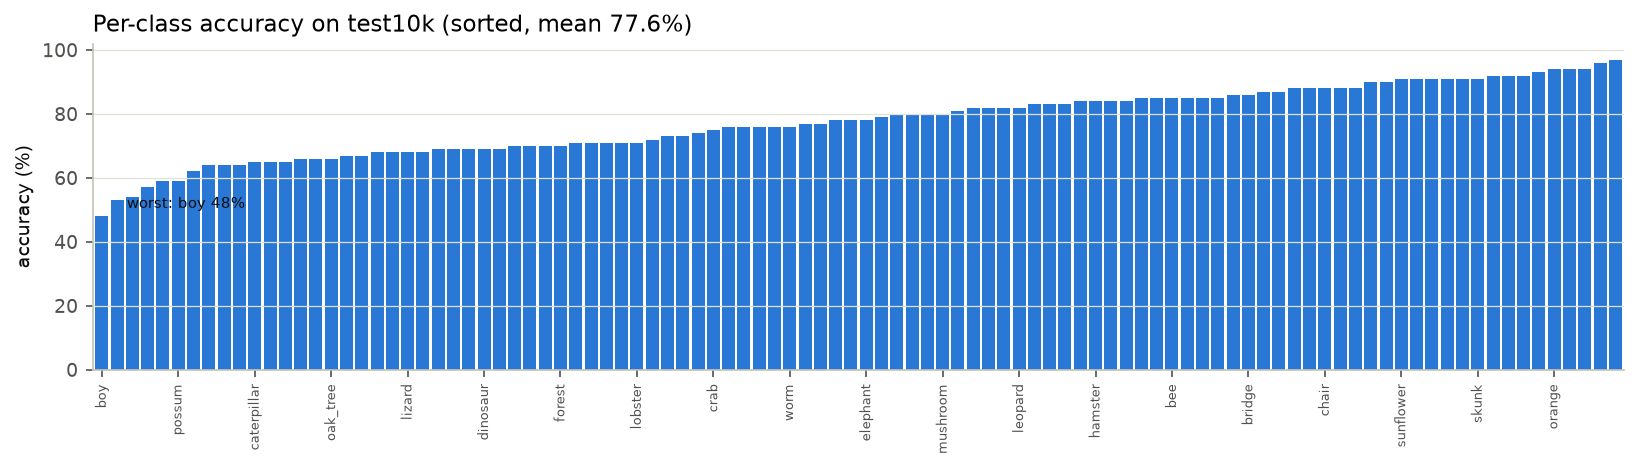
\includegraphics[width=0.99\linewidth]{per_class.png}
\caption{Fine-class accuracy for the three-model ensemble, sorted from lowest to highest. The mean is 77.6\%.}
\label{fig:per-class}
\end{figure}

Figure~\ref{fig:errors} complements the class-level plot with high-confidence mistakes. Several errors are visually understandable at $32\times32$: a lobster is predicted as a crab, a bicycle as a motorcycle, and a cup as a bottle. The model is therefore often confident about a plausible superclass or object family, but its fine label is not always recoverable from the pixels.

\begin{figure}[htbp]
\centering
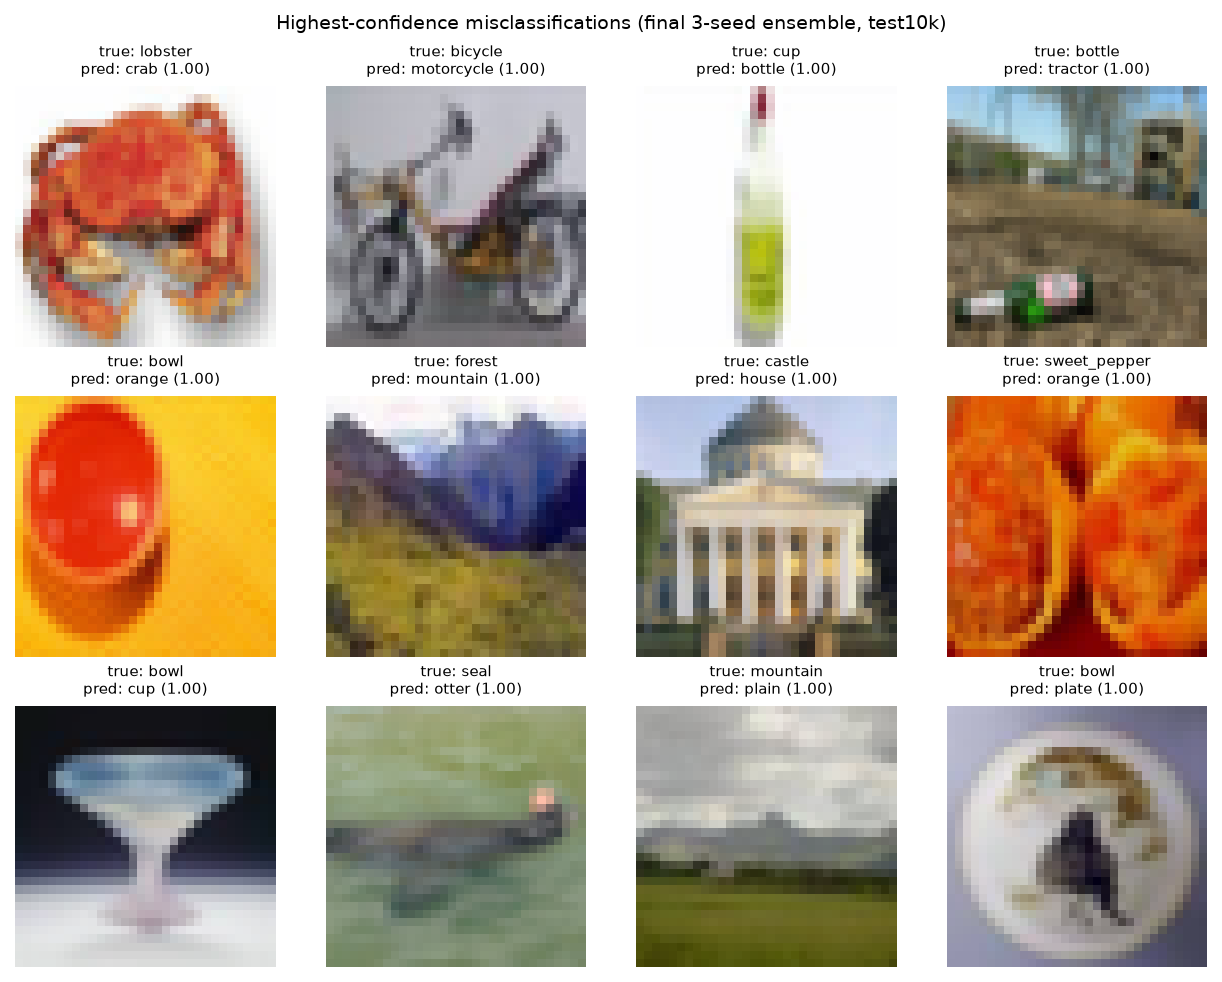
\includegraphics[width=0.92\linewidth]{error_samples.png}
\caption{Examples of high-confidence errors from the final ensemble. Each title gives the true class, predicted class, and confidence.}
\label{fig:errors}
\end{figure}

\section{What I Learned from Part A}

\begin{enumerate}
    \item \textbf{Stability can dominate optimizer choice.} Adam alone improved the mean over SGD but produced a 0.76\% seed. BatchNorm changed that unstable regime into a repeatable 47.17\% result. A large mean without a stability check can therefore be misleading.
    \item \textbf{The value of augmentation depends on the training budget.} Crop-and-flip was 4.16 points worse at ten epochs, yet 11.01 and 13.33 points better for the wide and deep-residual models at 60 epochs. The early loss is a regularization delay, not evidence that the transform is intrinsically harmful.
    \item \textbf{Capacity should be spent where the data can use it.} Width produced the strongest single architectural gain. Depth alone reduced accuracy by 3.11 points at 20 epochs, but adding residual connections recovered the loss and produced a positive 1.52-point change in the replicated comparison. The residual path made additional depth trainable rather than automatically useful.
    \item \textbf{Small improvements need replication.} A one-point difference appeared between repeated runs with the same nominal configuration because worker-side augmentation randomness was not controlled by the main-process seed. This made the three-seed confirmations more informative than a single best run and prevented treating sub-point changes as firm conclusions.
    \item \textbf{Error structure is informative.} More than one third of the final errors stay inside one superclass, far above the random reference. The remaining problem is therefore fine-grained discrimination among related categories, which suggests that better local features or higher-resolution information would be more promising than another blind increase in depth.
\end{enumerate}

\clearpage
\section*{Part B: Neural Network from Scratch}
\setcounter{section}{0}
\renewcommand{\thesection}{B.\arabic{section}}

This part is reserved for the NumPy-only implementation and its comparison with the PyTorch reference. The final article will use the following structure so that the implementation, verification, and end-to-end experiment remain separate from Part A.

\section{Overview and Constraints}
\label{sec:partb-overview}
Dataset protocol, numerical restrictions, and the design of the from-scratch training pipeline.

\section{Implementation Discipline}
\label{sec:partb-discipline}
Package structure, reproducibility controls, numerical checks, and the separation between the NumPy implementation and the reference implementation.

\section{Module Implementations}
\label{sec:partb-modules}
\subsection{GELU}
\subsection{Linear}
\subsection{Cross-Entropy Loss}
\subsection{Adam}
\subsection{Conv2d}
\subsection{SwitchNorm2d}
\subsection{Module Verification Summary}

\section{End-to-End Training and Comparison}
\label{sec:partb-training}
Network architecture, training curves, numerical agreement with PyTorch, accuracy comparison, and runtime analysis.

\section{What I Learned from Part B}
\label{sec:partb-learned}
Evidence-based conclusions from the manual forward and backward implementations.

\section*{References}

\begin{thebibliography}{9}
\bibitem{krizhevsky}
A. Krizhevsky, ``Learning Multiple Layers of Features from Tiny Images,'' technical report, University of Toronto, 2009.

\bibitem{batchnorm}
S. Ioffe and C. Szegedy, ``Batch Normalization: Accelerating Deep Network Training by Reducing Internal Covariate Shift,'' in \emph{Proceedings of ICML}, 2015.

\bibitem{adam}
D. P. Kingma and J. Ba, ``Adam: A Method for Stochastic Optimization,'' in \emph{Proceedings of ICLR}, 2015.

\bibitem{resnet}
K. He, X. Zhang, S. Ren, and J. Sun, ``Deep Residual Learning for Image Recognition,'' in \emph{Proceedings of CVPR}, 2016.

\bibitem{sgdr}
I. Loshchilov and F. Hutter, ``SGDR: Stochastic Gradient Descent with Warm Restarts,'' in \emph{Proceedings of ICLR}, 2017.

\bibitem{pytorch}
A. Paszke et al., ``PyTorch: An Imperative Style, High-Performance Deep Learning Library,'' in \emph{Advances in Neural Information Processing Systems}, 2019.
\end{thebibliography}

\end{document}
